\section{QuickDough Framework}\label{sec:framework}

\subsection{System Context}
This work assumes a hybrid computing architecture with a host processor and an FPGA accelerator, where the processor handles tasks not-well suited to FPGA such as providing the OS environment and FPGA focuses on compute intensive kernels.

Figure \ref{fig:typical-FPGA-accelerator} shows a typical FPGA acceleration architecture and all the experiments in this work stick to it. In this system, FPGA accelerator is attached to the system bus and it could access main memory through the bus. Inner the FPGA accelerator, there is a group of data buffers, an acceleration control block(Acc Ctrl), and a computation core. Data buffers are employed to store input data, output data and even temporary data of the computation. The Acc Ctrl block receives computation start signal probably from CPU via the bus when the input data is ready. Then it will trigger the computation core to start computation. When the computation is done, it will send the computation done signal back to interrupt CPU to collect data from the output buffer. The computation core is a customized circuit optimized for target compute kernel, which is supposed to be fast.  

\begin{figure}[H]
    \center{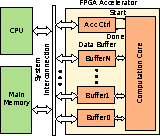
\includegraphics[width=0.5\linewidth]{typical-FPGA-accelerator}}
    \caption{A Typical FPGA Acceleration Architecture}
    \label{fig:typical-FPGA-accelerator}
\end{figure}

\subsection{QuickDough}
In this section, QuickDough, which is developed to provide a customized acceleration solution to the target applications based on such a acceleration architecture, is presented. As shown in Figure \ref{fig:framework}, it starts from HW/SW partition where the compute intensive kernels of the applications are extracted. The extracted kernels are further transformed to DFGs, which are preferred in CGRA compilation. There are already work on both, which may help us to automate the processing \cite{Baleani2002HW-SW} \cite{ROCCC}. Currently, we just manually perform the HW/SW partition and DFG transformation in our preliminary research stage. 

After the HW/SW partition, the design method can roughly be split into two parts. The part on top half is essentially the conventional software compilation except that we need to replace the compute kernel with accelerator drivers to mange the accelerator in the application, and the binary code is generated in the end. The part on the bottom half is basically the SCGRA compilation. Given the DFG of the compute kernel and accelerator configuration such as SCGRA size and on chip buffer capacity, the SCGRA compiler performs the operation scheduling, produces the configurations of the SCGRA overlay and generates the bitstream eventually based on the pre-implemented SCGRA overlay in the SCGRA library. Finally, the binary code is loaded to the host system, the bitstream is configured to FPGA and the application is implemented on the hybrid compute system. 

\begin{figure}[H]
    \center{\includegraphics[width=0.9\linewidth]{framework}}
    \caption{QuickDough: An FPGA Accelerator Design Method Using SCGRA Overlay}
    \label{fig:framework}
\end{figure}

